% Options for packages loaded elsewhere
\PassOptionsToPackage{unicode}{hyperref}
\PassOptionsToPackage{hyphens}{url}
%
\documentclass[
]{book}
\usepackage{amsmath,amssymb}
\usepackage{lmodern}
\usepackage{iftex}
\ifPDFTeX
  \usepackage[T1]{fontenc}
  \usepackage[utf8]{inputenc}
  \usepackage{textcomp} % provide euro and other symbols
\else % if luatex or xetex
  \usepackage{unicode-math}
  \defaultfontfeatures{Scale=MatchLowercase}
  \defaultfontfeatures[\rmfamily]{Ligatures=TeX,Scale=1}
\fi
% Use upquote if available, for straight quotes in verbatim environments
\IfFileExists{upquote.sty}{\usepackage{upquote}}{}
\IfFileExists{microtype.sty}{% use microtype if available
  \usepackage[]{microtype}
  \UseMicrotypeSet[protrusion]{basicmath} % disable protrusion for tt fonts
}{}
\makeatletter
\@ifundefined{KOMAClassName}{% if non-KOMA class
  \IfFileExists{parskip.sty}{%
    \usepackage{parskip}
  }{% else
    \setlength{\parindent}{0pt}
    \setlength{\parskip}{6pt plus 2pt minus 1pt}}
}{% if KOMA class
  \KOMAoptions{parskip=half}}
\makeatother
\usepackage{xcolor}
\usepackage{color}
\usepackage{fancyvrb}
\newcommand{\VerbBar}{|}
\newcommand{\VERB}{\Verb[commandchars=\\\{\}]}
\DefineVerbatimEnvironment{Highlighting}{Verbatim}{commandchars=\\\{\}}
% Add ',fontsize=\small' for more characters per line
\usepackage{framed}
\definecolor{shadecolor}{RGB}{248,248,248}
\newenvironment{Shaded}{\begin{snugshade}}{\end{snugshade}}
\newcommand{\AlertTok}[1]{\textcolor[rgb]{0.94,0.16,0.16}{#1}}
\newcommand{\AnnotationTok}[1]{\textcolor[rgb]{0.56,0.35,0.01}{\textbf{\textit{#1}}}}
\newcommand{\AttributeTok}[1]{\textcolor[rgb]{0.77,0.63,0.00}{#1}}
\newcommand{\BaseNTok}[1]{\textcolor[rgb]{0.00,0.00,0.81}{#1}}
\newcommand{\BuiltInTok}[1]{#1}
\newcommand{\CharTok}[1]{\textcolor[rgb]{0.31,0.60,0.02}{#1}}
\newcommand{\CommentTok}[1]{\textcolor[rgb]{0.56,0.35,0.01}{\textit{#1}}}
\newcommand{\CommentVarTok}[1]{\textcolor[rgb]{0.56,0.35,0.01}{\textbf{\textit{#1}}}}
\newcommand{\ConstantTok}[1]{\textcolor[rgb]{0.00,0.00,0.00}{#1}}
\newcommand{\ControlFlowTok}[1]{\textcolor[rgb]{0.13,0.29,0.53}{\textbf{#1}}}
\newcommand{\DataTypeTok}[1]{\textcolor[rgb]{0.13,0.29,0.53}{#1}}
\newcommand{\DecValTok}[1]{\textcolor[rgb]{0.00,0.00,0.81}{#1}}
\newcommand{\DocumentationTok}[1]{\textcolor[rgb]{0.56,0.35,0.01}{\textbf{\textit{#1}}}}
\newcommand{\ErrorTok}[1]{\textcolor[rgb]{0.64,0.00,0.00}{\textbf{#1}}}
\newcommand{\ExtensionTok}[1]{#1}
\newcommand{\FloatTok}[1]{\textcolor[rgb]{0.00,0.00,0.81}{#1}}
\newcommand{\FunctionTok}[1]{\textcolor[rgb]{0.00,0.00,0.00}{#1}}
\newcommand{\ImportTok}[1]{#1}
\newcommand{\InformationTok}[1]{\textcolor[rgb]{0.56,0.35,0.01}{\textbf{\textit{#1}}}}
\newcommand{\KeywordTok}[1]{\textcolor[rgb]{0.13,0.29,0.53}{\textbf{#1}}}
\newcommand{\NormalTok}[1]{#1}
\newcommand{\OperatorTok}[1]{\textcolor[rgb]{0.81,0.36,0.00}{\textbf{#1}}}
\newcommand{\OtherTok}[1]{\textcolor[rgb]{0.56,0.35,0.01}{#1}}
\newcommand{\PreprocessorTok}[1]{\textcolor[rgb]{0.56,0.35,0.01}{\textit{#1}}}
\newcommand{\RegionMarkerTok}[1]{#1}
\newcommand{\SpecialCharTok}[1]{\textcolor[rgb]{0.00,0.00,0.00}{#1}}
\newcommand{\SpecialStringTok}[1]{\textcolor[rgb]{0.31,0.60,0.02}{#1}}
\newcommand{\StringTok}[1]{\textcolor[rgb]{0.31,0.60,0.02}{#1}}
\newcommand{\VariableTok}[1]{\textcolor[rgb]{0.00,0.00,0.00}{#1}}
\newcommand{\VerbatimStringTok}[1]{\textcolor[rgb]{0.31,0.60,0.02}{#1}}
\newcommand{\WarningTok}[1]{\textcolor[rgb]{0.56,0.35,0.01}{\textbf{\textit{#1}}}}
\usepackage{longtable,booktabs,array}
\usepackage{calc} % for calculating minipage widths
% Correct order of tables after \paragraph or \subparagraph
\usepackage{etoolbox}
\makeatletter
\patchcmd\longtable{\par}{\if@noskipsec\mbox{}\fi\par}{}{}
\makeatother
% Allow footnotes in longtable head/foot
\IfFileExists{footnotehyper.sty}{\usepackage{footnotehyper}}{\usepackage{footnote}}
\makesavenoteenv{longtable}
\usepackage{graphicx}
\makeatletter
\def\maxwidth{\ifdim\Gin@nat@width>\linewidth\linewidth\else\Gin@nat@width\fi}
\def\maxheight{\ifdim\Gin@nat@height>\textheight\textheight\else\Gin@nat@height\fi}
\makeatother
% Scale images if necessary, so that they will not overflow the page
% margins by default, and it is still possible to overwrite the defaults
% using explicit options in \includegraphics[width, height, ...]{}
\setkeys{Gin}{width=\maxwidth,height=\maxheight,keepaspectratio}
% Set default figure placement to htbp
\makeatletter
\def\fps@figure{htbp}
\makeatother
\setlength{\emergencystretch}{3em} % prevent overfull lines
\providecommand{\tightlist}{%
  \setlength{\itemsep}{0pt}\setlength{\parskip}{0pt}}
\setcounter{secnumdepth}{5}
\usepackage{booktabs}
\ifLuaTeX
  \usepackage{selnolig}  % disable illegal ligatures
\fi
\usepackage[]{natbib}
\bibliographystyle{plainnat}
\IfFileExists{bookmark.sty}{\usepackage{bookmark}}{\usepackage{hyperref}}
\IfFileExists{xurl.sty}{\usepackage{xurl}}{} % add URL line breaks if available
\urlstyle{same} % disable monospaced font for URLs
\hypersetup{
  pdftitle={História da Psicologia},
  pdfauthor={Daniel Claudino},
  hidelinks,
  pdfcreator={LaTeX via pandoc}}

\title{História da Psicologia}
\author{Daniel Claudino}
\date{2022-10-14}

\usepackage{amsthm}
\newtheorem{theorem}{Theorem}[chapter]
\newtheorem{lemma}{Lemma}[chapter]
\newtheorem{corollary}{Corollary}[chapter]
\newtheorem{proposition}{Proposition}[chapter]
\newtheorem{conjecture}{Conjecture}[chapter]
\theoremstyle{definition}
\newtheorem{definition}{Definition}[chapter]
\theoremstyle{definition}
\newtheorem{example}{Example}[chapter]
\theoremstyle{definition}
\newtheorem{exercise}{Exercise}[chapter]
\theoremstyle{definition}
\newtheorem{hypothesis}{Hypothesis}[chapter]
\theoremstyle{remark}
\newtheorem*{remark}{Remark}
\newtheorem*{solution}{Solution}
\begin{document}
\maketitle

{
\setcounter{tocdepth}{1}
\tableofcontents
}
\hypertarget{sobre}{%
\chapter{Sobre}\label{sobre}}

Neste material, estão contidos os resumos de capítulos de livros, slides, notas de aula, apresentações, exercício respondidos em sala, atividades de revisão e questionários para as provas, além de outros materiais elaborados durante da disciplina

\hypertarget{histuxf3ria-da-psicologia}{%
\chapter{História da Psicologia}\label{histuxf3ria-da-psicologia}}

A disciplina tem como objetivo proporcionar ao aluno os conhecimentos em relação à História da Psicologia através de suas raízes filosóficas e fisiológicas, bem como a compreensão das diversas escolas e suas epistemologias. Também pretende-se oportunizar o entendimento das diversas complexidades que envolvem as teorias psicológicas e seus respectivos autores.

\hypertarget{professora}{%
\section*{Professor(a)}\label{professora}}
\addcontentsline{toc}{section}{Professor(a)}

\begin{itemize}
\tightlist
\item
  \textbf{Profª. Meª.} Eva Maria Lins Silva
\end{itemize}

\hypertarget{teste-referuxeancias}{%
\section{Teste Referências}\label{teste-referuxeancias}}

Each \textbf{bookdown} chapter \citep{book}

\hypertarget{notas-de-aula}{%
\chapter{Notas de Aula}\label{notas-de-aula}}

Neste capítulo estarão contidas todas as minhas notas de aula da disciplina História da Psicologia.

\hypertarget{professora-1}{%
\section*{Professor(a)}\label{professora-1}}
\addcontentsline{toc}{section}{Professor(a)}

\begin{itemize}
\tightlist
\item
  \textbf{Profª. Meª.} Eva Maria Lins Silva
\end{itemize}

\hypertarget{aula-01---a-histuxf3ria-da-psicologia}{%
\section{Aula 01 - A história da Psicologia}\label{aula-01---a-histuxf3ria-da-psicologia}}

\hypertarget{a-evoluuxe7uxe3o-da-ciuxeancia-psicologia}{%
\subsection*{A Evolução da Ciência Psicologia}\label{a-evoluuxe7uxe3o-da-ciuxeancia-psicologia}}
\addcontentsline{toc}{subsection}{A Evolução da Ciência Psicologia}

\hypertarget{psicologia-e-histuxf3ria}{%
\subsection*{Psicologia e História}\label{psicologia-e-histuxf3ria}}
\addcontentsline{toc}{subsection}{Psicologia e História}

Para \protect\hyperlink{bibliografia}{BOCK, FURTADO e TEIXEIRA (2011, p.31)}\textsuperscript{1}, tornamo-nos pouco compreensíveis se não recorrermos a \textbf{nossa história} e a \textbf{nossa perspectiva de futuro} para entendermos quem somos e para entendermos por que somos o que somos.

Segundo \protect\hyperlink{bibliografia}{DAVIDOFF (2001, p.8)}\textsuperscript{2}, desde os tempos ancestrais, o homem tem buscado entender a si próprio e aos outros.

Para compreender a ==diversidade== com que ==a Psicologia se apresenta hoje==, na busca por essa compreensão do homem, é indispensável \textbf{recuperar a sua história} \protect\hyperlink{bibliografia}{BOCK, FURTADO e TEIXEIRA (2011, p.31)}\textsuperscript{1}

\hypertarget{a-psicologia-entre-os-gregos}{%
\subsection*{A psicologia entre os Gregos}\label{a-psicologia-entre-os-gregos}}
\addcontentsline{toc}{subsection}{A psicologia entre os Gregos}

Na antiguidade, os gregos foram um dos povos mais evoluídos do seu tempo de forma que eles deixaram sua marca na história do pensamento humano.

As cidades-estado gregas proporcionaram a riqueza e o crescimento que exigiam soluções práticas para vários aspectos da vida cotidiana grega, inclusive para a organização social. Isso implicou avanços na teoria política, a invenção da democracia, entre outras conquistas que deixaram um legado para a humanidade.

Uma das primeiras tentativas de sistematiza conhecimentos a respeito do homem e sua interioridade teve contribuições gregas. Dessa tentativa, deixou-se o legado:

\begin{itemize}
\tightlist
\item
  De \emph{Psyché} como a palavra grega que significava \textbf{alma}. Para essa alma era dedicado um estudo (\emph{logos}), daí a origem da palavra usada até hoje, \textbf{psicologia}. Para os gregos, psicologia era o estudo da \textbf{alma};
\item
  De \emph{logos} que significa \textbf{razão}, além de significar estudo quando justaposta a outra palavra;
\item
  Para os gregos, \textbf{alma} e \textbf{espírito} ==era a mesma ==e era neles que ==se situavam==:

  \begin{itemize}
  \tightlist
  \item
    os sentimentos;
  \item
    o pensamento;
  \item
    a irracionalidade;
  \item
    o desejo;
  \item
    a sensação
  \item
    a \textbf{percepção} ( era a relação do homem com o mundo );
  \end{itemize}
\item
  Entre os gregos, havia uma ==oposição== entre \textbf{idealismo} (o mundo é concebido primeiro dentro do homem, daí ele passa a existir) e \textbf{materialismo} (o mundo existe primeiro, daí o homem o percebe)
\end{itemize}

\hypertarget{para-suxf3crates}{%
\subsubsection*{Para Sócrates}\label{para-suxf3crates}}
\addcontentsline{toc}{subsubsection}{Para Sócrates}

\begin{itemize}
\tightlist
\item
  \textbf{Principal preocupação}: O ==limite== que separa os \textbf{homens} dos \textbf{animais};
\item
  A ==razão== permite ao homem sobrepor os \textbf{instintos} (base para a irracionalidade);
\item
  A ==razão== é a ==essência== da humanidade ( Esse é um caminho aberto por Sócrates que será muito explorado pela psicologia);
\item
  As ==teorias da consciência== são, de certa forma, frutos dessa primeira sistematização da Filosofia.
\end{itemize}

\hypertarget{para-platuxe3o}{%
\subsubsection*{Para Platão}\label{para-platuxe3o}}
\addcontentsline{toc}{subsubsection}{Para Platão}

\begin{itemize}
\tightlist
\item
  \textbf{Principal preocupação}: Definir um ==lugar== para a \textbf{razão} em nosso corpo ( a cabeça );
\item
  A ==cabeça== era o lugar da \textbf{razão} e da \textbf{alma};
\item
  A ==medula== era um ==elemento de ligação== entre a \textbf{alma} e o \textbf{corpo};
\item
  Concebia a \textbf{ALMA} ==separada== do \textbf{CORPO};
\item
  Quando alguém morria:

  \begin{itemize}
  \tightlist
  \item
    O ==corpo== desaparecia;
  \item
    A ==alma== ficava livre para ocupar outro corpo;
  \end{itemize}
\end{itemize}

\hypertarget{para-aristuxf3teles}{%
\subsubsection*{Para Aristóteles}\label{para-aristuxf3teles}}
\addcontentsline{toc}{subsubsection}{Para Aristóteles}

\begin{itemize}
\tightlist
\item
  No pensamento grego, foi o ==primeiro que postulou== que ==a ALMA e o CORPO \textbf{NÃO podem ser dissossiados}==.;
\item
  \emph{Psyché} era o ==princípio ativo da vida==;
\item
  Possui \emph{Psyché} (alma): Quem (1) cresce, (2) se reproduz, (3) se alimenta (homens, vegetais e animais);

  \begin{itemize}
  \tightlist
  \item
    Alma ==vegetativa==(vegetais): se reproduz / se alimenta;
  \item
    Alma ==sensitiva==(animais): percepção / movimento
  \item
    Alma ==racional==(homem): se reproduz / se alimenta / percepção / movimento
  \end{itemize}
\item
  Esse filósofo estudou a ==diferença== entre \textbf{razão}, \textbf{percepção} e \textbf{sensação}.
\end{itemize}

\hypertarget{resumo-das-teorias-gregas-sobre-a-psicologia}{%
\subsubsection*{Resumo das teorias gregas sobre a Psicologia}\label{resumo-das-teorias-gregas-sobre-a-psicologia}}
\addcontentsline{toc}{subsubsection}{Resumo das teorias gregas sobre a Psicologia}

\begin{itemize}
\tightlist
\item
  \textbf{Platônica}: A imortalidade da ==ALMA== e sua ==\textbf{SEPARAÇÃO DO CORPO}==;
\item
  \textbf{Aristotélica}: Da mortalidade da ==ALMA== e da sua relação de ==\textbf{PERTENCIMENTO AO CORPO}==;
\end{itemize}

\hypertarget{a-psicologia-na-idade-muxe9dia}{%
\subsection*{A psicologia na Idade Média}\label{a-psicologia-na-idade-muxe9dia}}
\addcontentsline{toc}{subsection}{A psicologia na Idade Média}

Na antiguidade, após a dominação da Grécia pelos romanos e após o surgimento do cristianismo tornando-se a principal religião da idade média, dois filósofos destacam-se em relação ao ==estudo do psiquismo==.

\hypertarget{santo-agostinho}{%
\subsubsection*{Santo Agostinho}\label{santo-agostinho}}
\addcontentsline{toc}{subsubsection}{Santo Agostinho}

\begin{itemize}
\tightlist
\item
  Fazia \textbf{SEPARAÇÃO} entre alma e corpo;
\item
  \textbf{Alma}: (1) Sede da ==razão== e do ==pensamento== / (2) ==prova da manifestação divina== no homem / (3) ==imortal== / (4) Elemento que ==liga o homem a Deus==;
\end{itemize}

A Igreja passa a se preocupar com a alma enquanto sede do pensamento.

\hypertarget{suxe3o-tomaz-de-aquino}{%
\subsubsection*{São Tomaz de Aquino}\label{suxe3o-tomaz-de-aquino}}
\addcontentsline{toc}{subsubsection}{São Tomaz de Aquino}

A época em que São Tomaz de Aquino viveu foi marcada por diversas situações históricas importantes:

\begin{itemize}
\tightlist
\item
  Ruptura da Igreja Católica ( aparecimento do protestantismo );
\item
  Revolução Francesa;
\item
  Revolução Industrial ( na Inglaterra );
\end{itemize}

Essa situação teve como consequências:

\begin{itemize}
\tightlist
\item
  Crise na economia mundial e na sociedade;
\item
  ==Questionamento== (1) da Igreja e (2) dos conhecimentos produzidos por ela;
\item
  Procura por novas justificativas para a relação do homem com Deus;
\end{itemize}

Das questões filosóficas introduzidas pelos gregos, a distinção entre ==essência== e ==existência== foi trabalhada por São Tomaz de Aquino.
* \textbf{Partindo da ideia}: Que o homem, ==\textbf{na sua essência}==, busca a perfeição através de sua existência.
* \textbf{Afirma que}:
* Só Deus seria capaz de reunir ==essência== e ==existência==;
* A busca de perfeição pelo homem seria a busca de Deus;

\hypertarget{a-psicologia-no-renascimento}{%
\subsection*{A PSICOLOGIA NO RENASCIMENTO}\label{a-psicologia-no-renascimento}}
\addcontentsline{toc}{subsection}{A PSICOLOGIA NO RENASCIMENTO}

\hypertarget{a-origem-da-psicologia-cientuxedfica}{%
\subsection*{A ORIGEM DA PSICOLOGIA CIENTÍFICA}\label{a-origem-da-psicologia-cientuxedfica}}
\addcontentsline{toc}{subsection}{A ORIGEM DA PSICOLOGIA CIENTÍFICA}

\hypertarget{a-psicologia-cientuxedfica}{%
\subsection*{A PSICOLOGIA CIENTÍFICA}\label{a-psicologia-cientuxedfica}}
\addcontentsline{toc}{subsection}{A PSICOLOGIA CIENTÍFICA}

\hypertarget{o-funcionalismo}{%
\subsubsection*{O Funcionalismo}\label{o-funcionalismo}}
\addcontentsline{toc}{subsubsection}{O Funcionalismo}

\hypertarget{o-estruturalismo}{%
\subsubsection*{O Estruturalismo}\label{o-estruturalismo}}
\addcontentsline{toc}{subsubsection}{O Estruturalismo}

\hypertarget{associativismo}{%
\subsubsection*{Associativismo}\label{associativismo}}
\addcontentsline{toc}{subsubsection}{Associativismo}

\hypertarget{as-principais-teorias-da-psicologia-no-suxe9culo-20}{%
\subsection*{AS PRINCIPAIS TEORIAS DA PSICOLOGIA NO SÉCULO 20}\label{as-principais-teorias-da-psicologia-no-suxe9culo-20}}
\addcontentsline{toc}{subsection}{AS PRINCIPAIS TEORIAS DA PSICOLOGIA NO SÉCULO 20}

\hypertarget{o-behaviorismo}{%
\subsubsection*{O Behaviorismo}\label{o-behaviorismo}}
\addcontentsline{toc}{subsubsection}{O Behaviorismo}

Nasce com Watson e tem um desenvolvimento grande nos Estados Unidos, em função de suas aplicações práticas, tornou-se importante por ter definido o fato psicológico, de modo concreto, a partir da noção de comportamento (behavior).

\hypertarget{a-gestalt}{%
\subsubsection*{A Gestalt}\label{a-gestalt}}
\addcontentsline{toc}{subsubsection}{A Gestalt}

Surge na Europa como uma negação da fragmentação das ações e processos humanos, realizada pelas tendências da Psicologia científica do século 19, postulando a necessidade de se compreender o homem como uma totalidade. A Gestalt é a tendência teórica mais ligada à Filosofia.

\hypertarget{a-psicanuxe1lise}{%
\subsubsection*{A Psicanálise}\label{a-psicanuxe1lise}}
\addcontentsline{toc}{subsubsection}{A Psicanálise}

Nasce com Freud, na Áustria, a partir da prática médica, recupera para a Psicologia a importância da afetividade e postula o inconsciente como objeto de estudo, quebrando a tradição da Psicologia como ciência da consciência e da razão.

\hypertarget{cross}{%
\chapter{Cross-references}\label{cross}}

Cross-references make it easier for your readers to find and link to elements in your book.

\hypertarget{chapters-and-sub-chapters}{%
\section{Chapters and sub-chapters}\label{chapters-and-sub-chapters}}

There are two steps to cross-reference any heading:

\begin{enumerate}
\def\labelenumi{\arabic{enumi}.}
\tightlist
\item
  Label the heading: \texttt{\#\ Hello\ world\ \{\#nice-label\}}.

  \begin{itemize}
  \tightlist
  \item
    Leave the label off if you like the automated heading generated based on your heading title: for example, \texttt{\#\ Hello\ world} = \texttt{\#\ Hello\ world\ \{\#hello-world\}}.
  \item
    To label an un-numbered heading, use: \texttt{\#\ Hello\ world\ \{-\#nice-label\}} or \texttt{\{\#\ Hello\ world\ .unnumbered\}}.
  \end{itemize}
\item
  Next, reference the labeled heading anywhere in the text using \texttt{\textbackslash{}@ref(nice-label)}; for example, please see Chapter \ref{cross}.

  \begin{itemize}
  \tightlist
  \item
    If you prefer text as the link instead of a numbered reference use: \protect\hyperlink{cross}{any text you want can go here}.
  \end{itemize}
\end{enumerate}

\hypertarget{captioned-figures-and-tables}{%
\section{Captioned figures and tables}\label{captioned-figures-and-tables}}

Figures and tables \emph{with captions} can also be cross-referenced from elsewhere in your book using \texttt{\textbackslash{}@ref(fig:chunk-label)} and \texttt{\textbackslash{}@ref(tab:chunk-label)}, respectively.

See Figure \ref{fig:nice-fig}.

\begin{Shaded}
\begin{Highlighting}[]
\FunctionTok{par}\NormalTok{(}\AttributeTok{mar =} \FunctionTok{c}\NormalTok{(}\DecValTok{4}\NormalTok{, }\DecValTok{4}\NormalTok{, .}\DecValTok{1}\NormalTok{, .}\DecValTok{1}\NormalTok{))}
\FunctionTok{plot}\NormalTok{(pressure, }\AttributeTok{type =} \StringTok{\textquotesingle{}b\textquotesingle{}}\NormalTok{, }\AttributeTok{pch =} \DecValTok{19}\NormalTok{)}
\end{Highlighting}
\end{Shaded}

\begin{figure}

{\centering 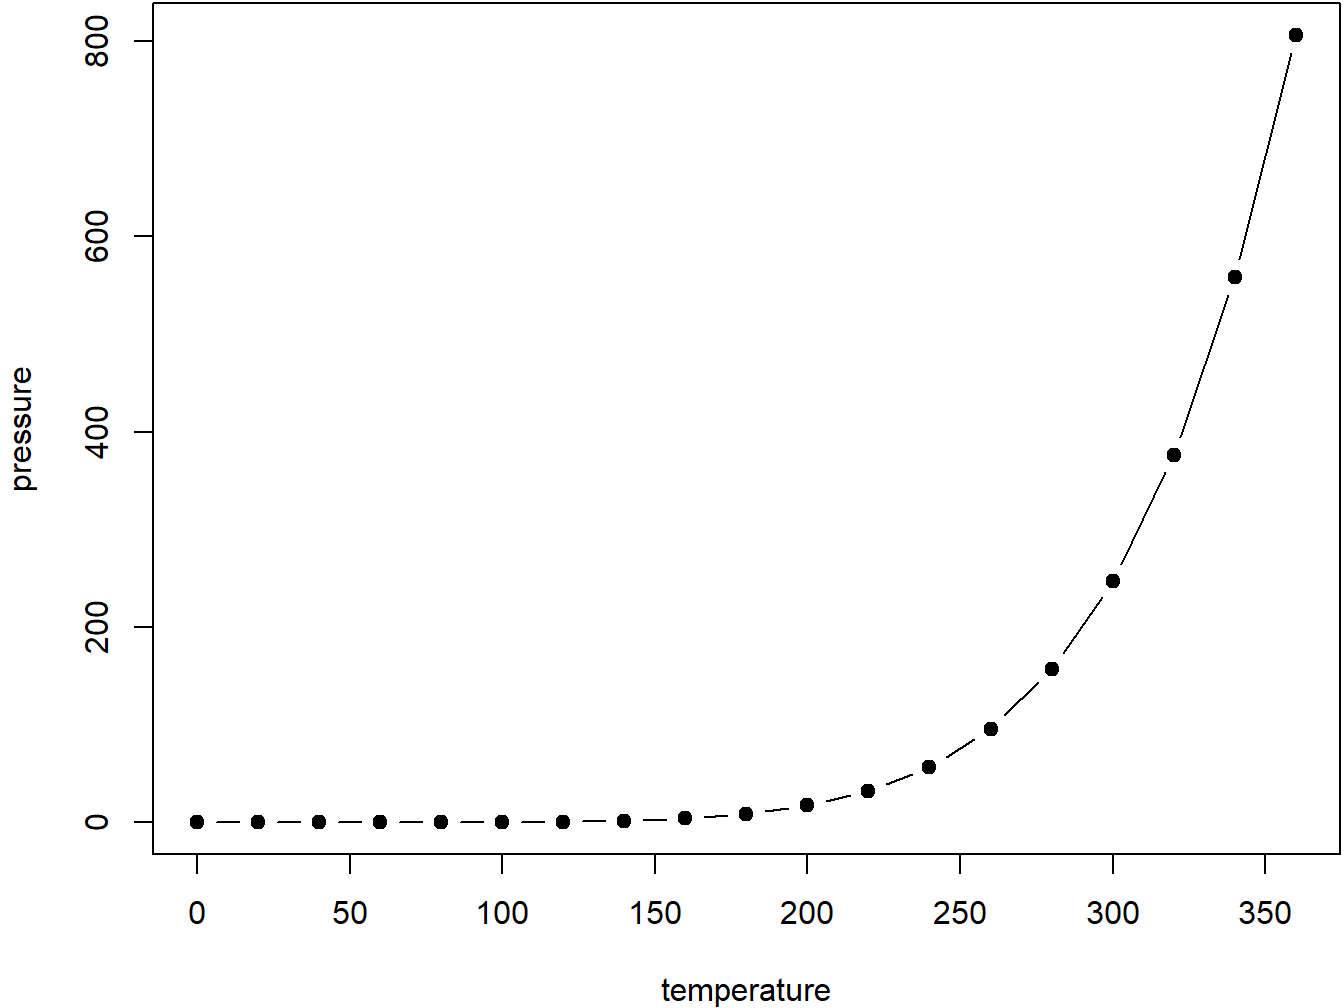
\includegraphics[width=0.8\linewidth]{_main_files/figure-latex/nice-fig-1} 

}

\caption{Here is a nice figure!}\label{fig:nice-fig}
\end{figure}

Don't miss Table \ref{tab:nice-tab}.

\begin{Shaded}
\begin{Highlighting}[]
\NormalTok{knitr}\SpecialCharTok{::}\FunctionTok{kable}\NormalTok{(}
  \FunctionTok{head}\NormalTok{(pressure, }\DecValTok{10}\NormalTok{), }\AttributeTok{caption =} \StringTok{\textquotesingle{}Here is a nice table!\textquotesingle{}}\NormalTok{,}
  \AttributeTok{booktabs =} \ConstantTok{TRUE}
\NormalTok{)}
\end{Highlighting}
\end{Shaded}

\begin{table}

\caption{\label{tab:nice-tab}Here is a nice table!}
\centering
\begin{tabular}[t]{rr}
\toprule
temperature & pressure\\
\midrule
0 & 0.0002\\
20 & 0.0012\\
40 & 0.0060\\
60 & 0.0300\\
80 & 0.0900\\
\addlinespace
100 & 0.2700\\
120 & 0.7500\\
140 & 1.8500\\
160 & 4.2000\\
180 & 8.8000\\
\bottomrule
\end{tabular}
\end{table}

\hypertarget{parts}{%
\chapter{Parts}\label{parts}}

You can add parts to organize one or more book chapters together. Parts can be inserted at the top of an .Rmd file, before the first-level chapter heading in that same file.

Add a numbered part: \texttt{\#\ (PART)\ Act\ one\ \{-\}} (followed by \texttt{\#\ A\ chapter})

Add an unnumbered part: \texttt{\#\ (PART\textbackslash{}*)\ Act\ one\ \{-\}} (followed by \texttt{\#\ A\ chapter})

Add an appendix as a special kind of un-numbered part: \texttt{\#\ (APPENDIX)\ Other\ stuff\ \{-\}} (followed by \texttt{\#\ A\ chapter}). Chapters in an appendix are prepended with letters instead of numbers.

\hypertarget{footnotes-and-citations}{%
\chapter{Footnotes and citations}\label{footnotes-and-citations}}

\hypertarget{footnotes}{%
\section{Footnotes}\label{footnotes}}

Footnotes are put inside the square brackets after a caret \texttt{\^{}{[}{]}}. Like this one \footnote{This is a footnote.}.

\hypertarget{citations}{%
\section{Citations}\label{citations}}

Reference items in your bibliography file(s) using \texttt{@key}.

For example, we are using the \textbf{bookdown} package \citep{R-bookdown} (check out the last code chunk in index.Rmd to see how this citation key was added) in this sample book, which was built on top of R Markdown and \textbf{knitr} \citep{xie2015} (this citation was added manually in an external file book.bib).
Note that the \texttt{.bib} files need to be listed in the index.Rmd with the YAML \texttt{bibliography} key.

The RStudio Visual Markdown Editor can also make it easier to insert citations: \url{https://rstudio.github.io/visual-markdown-editing/\#/citations}

\hypertarget{blocks}{%
\chapter{Blocks}\label{blocks}}

\hypertarget{equations}{%
\section{Equations}\label{equations}}

Here is an equation.

\begin{equation} 
  f\left(k\right) = \binom{n}{k} p^k\left(1-p\right)^{n-k}
  \label{eq:binom}
\end{equation}

You may refer to using \texttt{\textbackslash{}@ref(eq:binom)}, like see Equation \eqref{eq:binom}.

\hypertarget{theorems-and-proofs}{%
\section{Theorems and proofs}\label{theorems-and-proofs}}

Labeled theorems can be referenced in text using \texttt{\textbackslash{}@ref(thm:tri)}, for example, check out this smart theorem \ref{thm:tri}.

\begin{theorem}
\protect\hypertarget{thm:tri}{}\label{thm:tri}For a right triangle, if \(c\) denotes the \emph{length} of the hypotenuse
and \(a\) and \(b\) denote the lengths of the \textbf{other} two sides, we have
\[a^2 + b^2 = c^2\]
\end{theorem}

Read more here \url{https://bookdown.org/yihui/bookdown/markdown-extensions-by-bookdown.html}.

\hypertarget{callout-blocks}{%
\section{Callout blocks}\label{callout-blocks}}

The R Markdown Cookbook provides more help on how to use custom blocks to design your own callouts: \url{https://bookdown.org/yihui/rmarkdown-cookbook/custom-blocks.html}

\hypertarget{sharing-your-book}{%
\chapter{Sharing your book}\label{sharing-your-book}}

\hypertarget{publishing}{%
\section{Publishing}\label{publishing}}

HTML books can be published online, see: \url{https://bookdown.org/yihui/bookdown/publishing.html}

\hypertarget{pages}{%
\section{404 pages}\label{pages}}

By default, users will be directed to a 404 page if they try to access a webpage that cannot be found. If you'd like to customize your 404 page instead of using the default, you may add either a \texttt{\_404.Rmd} or \texttt{\_404.md} file to your project root and use code and/or Markdown syntax.

\hypertarget{metadata-for-sharing}{%
\section{Metadata for sharing}\label{metadata-for-sharing}}

Bookdown HTML books will provide HTML metadata for social sharing on platforms like Twitter, Facebook, and LinkedIn, using information you provide in the \texttt{index.Rmd} YAML. To setup, set the \texttt{url} for your book and the path to your \texttt{cover-image} file. Your book's \texttt{title} and \texttt{description} are also used.

This \texttt{gitbook} uses the same social sharing data across all chapters in your book- all links shared will look the same.

Specify your book's source repository on GitHub using the \texttt{edit} key under the configuration options in the \texttt{\_output.yml} file, which allows users to suggest an edit by linking to a chapter's source file.

Read more about the features of this output format here:

\url{https://pkgs.rstudio.com/bookdown/reference/gitbook.html}

Or use:

\begin{Shaded}
\begin{Highlighting}[]
\NormalTok{?bookdown}\SpecialCharTok{::}\NormalTok{gitbook}
\end{Highlighting}
\end{Shaded}


  \bibliography{referencias.bib,packages.bib}

\end{document}
